\label{Architektur}
Im Fogenden soll ein Überblick über das Projekt vermittelt werden.
Hierzu werden die Anforderungen und schließlich die daraus resultierende Softwarearchitektur vorgestellt.

\subsection{Anforderungen}
Das Endresultat soll ein Programm sein, mit dem der Ersteller mühelos einen Online-Self-Assessment-Test generieren kann. 
Besonderes Augenmerk liegt dabei auf der leichten Bedienbarkeit.

Folgende Anforderungen werden an den Aufbau der Fragen gestellt:
\begin{itemize}
	\item Der Test soll aus Multiple-Choice-Fragen bestehen.
	\item Die Fragen und Antworten  sollen Text, Bilder und Videos enthalten können.
	\item Die Bearbeitungszeit jeder Frage soll optional beschränkt sein.
	\item Die Fragen sollen in Kategorien gegliedert werden können.
	\item Es soll einen Forschrittsbalken geben, welcher anzeigt wie viele Fragen bereits beantwortet wurden und wie viele noch zu beantworten sind.
\end{itemize}

Damit die Studieninteressierten Feedback erhalten können, muss am Ende eine Bewertung der eingegebenen Antworten durchgeführt werden.
Für diese Bewertung gelten folgende Anforderungen:
\begin{itemize}
	\item Die Gewichtung einer Frage soll vom Ersteller durch Angabe von Punkten festgelegt werden können.
	\item Für jede Kategorie soll die Anzahl der richtig beziehungsweise falsch beantworteten Fragen angezeigt werden.
	\item Basierend auf der erreichten Gesamtpunktzahl soll ein vom Ersteller gewähltes Feedback gegeben werden.
\end{itemize}

\subsection{Programmaufbau}
Abbildung~\ref{fig:umlCD} zeigt die implementierte Klassenstruktur.

\begin{figure*}
	 \centering
	 \caption{UML Klassendiagramm des Testgenerators}
	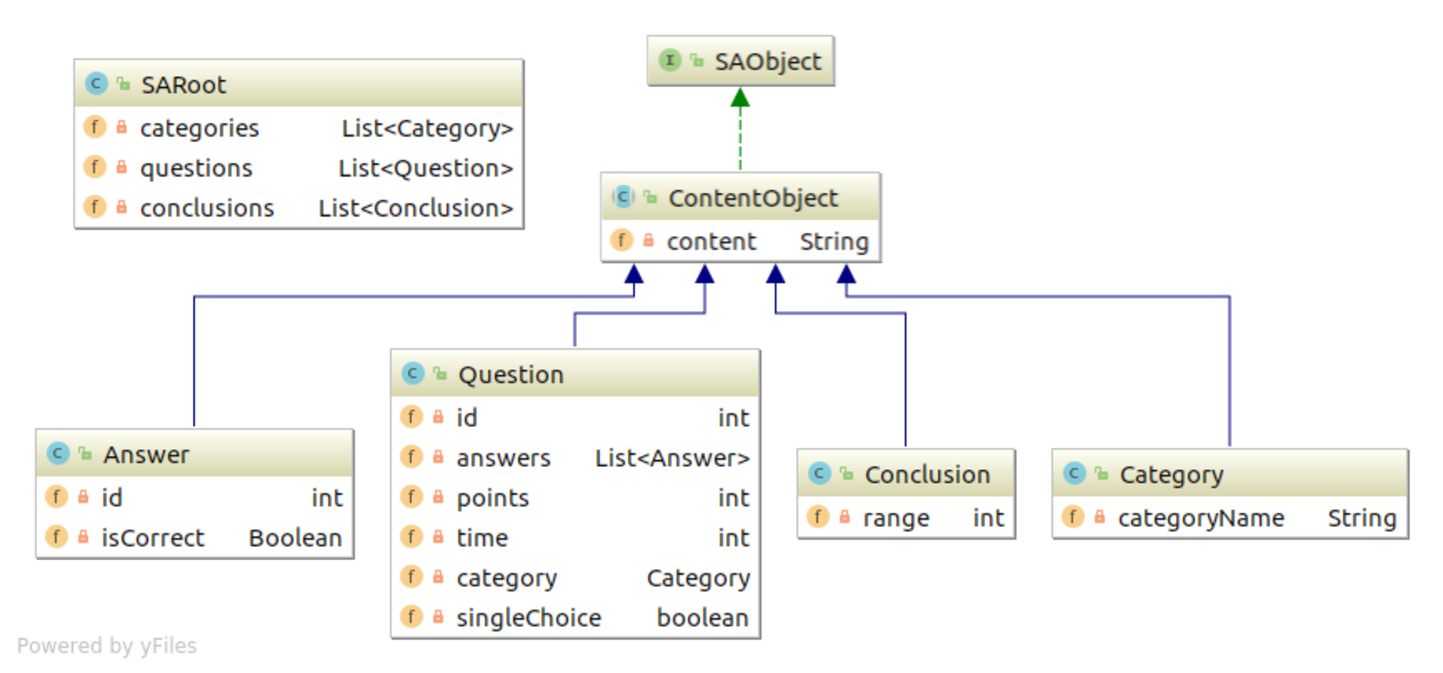
\includegraphics[width = \textwidth]{domain-class-diagram.pdf}
	\label{fig:umlCD}
\end{figure*}

Mit Hilfe der 'Creator'-Benutzeroberfläche, beschrieben in Abschnitt~\ref{Julian}, kann man Objekte der im Klassendiagramm dargestellten Klassen instanziieren. 
So kann der Ersteller einen Test modellieren.
Aus diesen Objekten kann schließlich direkt eine Webseite generiert werden. 
Die Beschreibung des Generators kann Abschnitt~\ref{Sokol} entnommen werden.

Der Parser, dokumentiert in Abschnitt~\ref{Tim}, bietet die Möglichkeit, die erstellten Objekte in einer XML-Datei zu speichern und sie wieder einzulesen.

Der Aufbau der generierten Webseite wird in Abschnitt~\ref{Jena} beschrieben.



